\documentclass[border=10pt]{standalone}
\usepackage{tikz}
\begin{document}
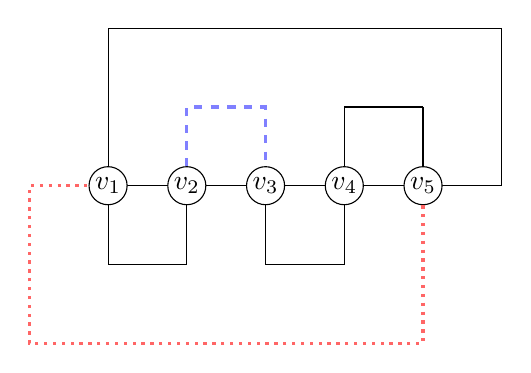
\begin{tikzpicture}
\draw (0, 0) -- (1, 0) -- (2, 0) -- (3, 0) -- (4, 0) -- (5, 0) -- (5,
2) -- (0, 2) -- (0, 0) -- (0, -1) -- (1, -1);
\draw (2,0) -- (2, -1) -- (3, -1) -- (3, 0) -- (3, 1) -- (4, 1);


\draw (0, 0.2) -- (0, -0.2);
\node[circle, fill=white, draw=black, inner sep=1pt] (v1) at (0, 0)
{ $v_1$};



\draw (0.8, 0) -- (1.2, 0);

\node[circle, fill=white, draw=black, inner sep=1pt] (v2) at (1, 0)
{ $v_2$};





\draw (2, 0.2) -- (2, -0.2);

\node[circle, fill=white, draw=black, inner sep=1pt] (v3) at (2, 0)
{ $v_3$};

\draw (2.8, 0) -- (3.2, 0);

\node[circle, fill=white, draw=black, inner sep=1pt] (v4) at (3, 0)
{ $v_4$};

\node[circle, fill=white, draw=black, inner sep=1pt] (v5) at (4, 0)
{ $v_5$};

\draw[, red!60!white, very thick, dotted] (v5) -- (4, -2) --
(-1, -2) -- (-1, 0) -- (v1);

\draw[, blue!50!white, very thick, dashed] (v2) -- (1, 1) -- (2,
1) -- (v3);

\draw[] (v1) -- (v2);
\draw[] (v2) -- (v3);
\draw[] (v3) -- (v4);
\draw[] (v4) -- (v5);
\draw[] (4,1) -- (v5);
\draw[] (3,-1) -- (v4);
\draw[] (1,-1) -- (v2);
\draw[] (0,1) -- (v1);

\end{tikzpicture}
\end{document}
